\documentclass[journal,12pt,twocolumn]{IEEEtran}
\usepackage{amsmath,amssymb,amsfonts,amsthm}
\usepackage{txfonts}
\usepackage{tkz-euclide}
\usepackage[margin=0.25in]{geometry}
\usepackage{pgfplots}
\usepackage{listings}
\usepackage{gvv}
\usepackage[latin1]{inputenc}
\usepackage{adjustbox}
\usepackage{array}
\usepackage{tabularx}
\usepackage{enumitem}
\usepackage{pgf}
\usepackage{lmodern}
\usepackage{circuitikz}
\usepackage{tikz}
\usepackage{graphicx}
\pgfplotsset{width=10cm,compat=1.18}

\begin{document}
\bibliographystyle{IEEEtran}

\vspace{3cm}

\title{}
\author{EE23BTECH11054 -  Sai Krishna Shanigarapu$^{*}$
}
\maketitle
\newpage
\bigskip

\section*{Gate MA 2022}
14. \hspace{2pt} The value of the integral 
\begin{align*}
    \int_C \frac{z^{100}}{z^{101}+1}\, dz
\end{align*}
where $C$ is the circle of radius 2 centred at the origin taken in the anti-clockwise direction is\\
\begin{enumerate}[label=(\Alph*)]
    \item $-2 \pi i$
    \item $2\pi$
    \item $0$
    \item $2\pi i $
\end{enumerate}
\hfill(GATE 2022 MA)\\
\solution\\

Cauchy's Theorem:\\
From Figure \ref{fig:fig1_gate_2022_ma_14}
\begin{align}
    \int_C f\brak{z}dz &= \int_{Cr} f\brak{z}dz
\end{align}
\begin{figure}[ht]
    \centering
    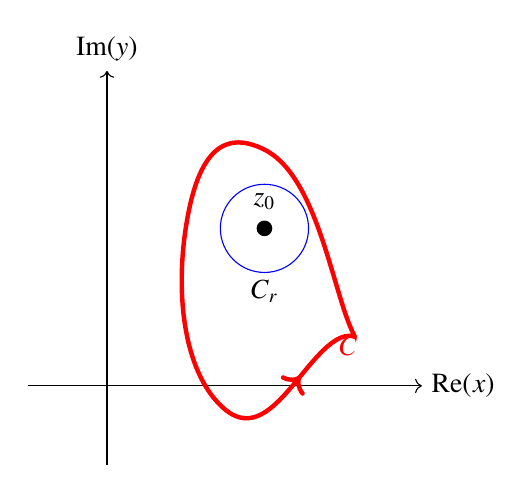
\begin{tikzpicture}
    % Real axis
    \draw[->] (-1,0) -- (4,0) node[right] {$\text{Re}(x)$};
    % Imaginary axis
    \draw[->] (0,-1) -- (0,4) node[above] {$\text{Im}(y)$};
    % Closed curve
    \draw[red, ultra thick, postaction={decorate,decoration={markings,mark=at position 0.6 with {\arrow{>}}}}] plot[smooth cycle, tension=1] coordinates {(3,1)  (2,3) (1,2) (1.5,-0.3) (2.8, 0.5)} node[right] {$C$};
    \node[circle,fill,inner sep=2pt,label={$z_0$}] at (2,2) {};
    \draw[color=blue] (2,2) circle [radius=0.56]; 
     \node at (2,1.2) {$C_r$};
\end{tikzpicture}

    \caption{Figure1}
    \label{fig:fig1_gate_2022_ma_14}
\end{figure}\\
Since  $g\brak{z}$ is continuous we know that $\abs{g\brak{z}}$ is bounded inside  $C_r$. Say,  $\abs{g\brak{z}}<M$. The corollary to the triangle inequality says that
\begin{align}
    \abs{\int_{C_r}f\brak{z}\, dz} &\leq M2\pi r.
\end{align}
Since  $r$ can be as small as we want, this implies that
\begin{align}
    \int_{Cr} f\brak{z}dz &= 0
\end{align}
let \begin{align}
    g\brak{z} &= \frac{f\brak{z} - f\brak{z_0}}{z-z_0}\\
    \lim_{z \to z_0} g(z) &= f'(z_0)\\
    \int_{C} g(z)\ dz = 0, &\implies \int_C \frac{f(z) - f(z_0)}{z - z_0} \ dz = 0
\end{align}
Thus,
\begin{align}
    \int_{C} \frac{f(z)}{z - z_0}\ dz = \int_C \dfrac{f(z_0)}{z - z_0}\ dz = 2\pi i f(z_0) \label{eq:eq3_gate_2022_ma_14}
\end{align}

Using Cauchy's Theorem,
\begin{align}
    \int_C f\brak{z} &= 0\\
    f\brak{a} &= \frac{1}{2 \pi i}\oint_C\frac{f\brak{z}}{z-a}\, dz\\
    f^{n}\brak{a} &= \frac{n!}{2 \pi i}\oint_C\frac{f\brak{z}}{\brak{z-a}^{n+1}}\, dz
\end{align}

Residue Theorem:\\
From eq (\ref{eq:eq3_gate_2022_ma_14})
\begin{align}
    \int_C f\brak{z}\, dz &= 2 \pi i \sum{Res \, f\brak{a}} \label{eq:eq1_gate_ma_2022_14_054}
\end{align}
where, for n repeated poles,
\begin{align}
    Res \, f\brak{a} &= \lim_{z \to a}\frac{1}{\brak{n-1}!}\brak{\frac{d^{n-1}}{dz^{n-1}}\sbrak{\brak{z-a}^n\, f\brak{z}}} \label{eq:eq2_gate_ma_2022_14_054}
\end{align}

Solving the integral,
\begin{align}
f\brak{z} &= \int_C \frac{z^{100}}{z^{101}+1}\, dz
\end{align}

\begin{figure}[ht]
    \centering
    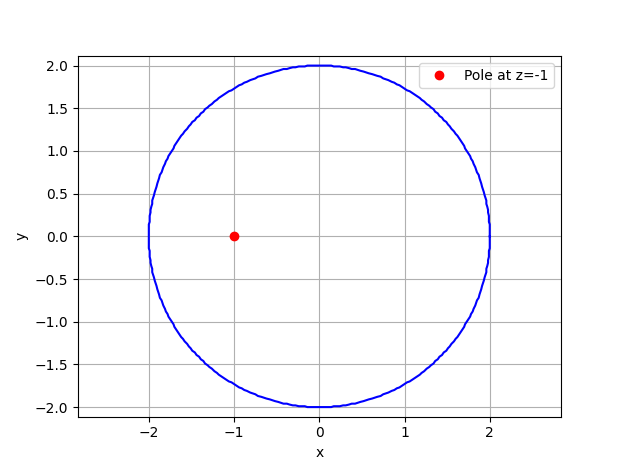
\includegraphics[width=\columnwidth]{figs/Figure_1.png}
    \caption{plot of $C$ with it's pole}
    \label{fig:fig1_gate_ma_2022_14_054}
\end{figure}
Since the pole $z=-1$ is inside the circle, Using eq (\ref{eq:eq2_gate_ma_2022_14_054})
\begin{align}
    Res\, f\brak{-1} &= \lim_{z\to -1}\brak{\frac{z^{100}}{z^{101}+1}}\brak{z^{101} + 1}\\
    &= 1 \label{eq:eq3_gate_ma_2022_14_054}
\end{align}

From eq (\ref{eq:eq1_gate_ma_2022_14_054}), and eq (\ref{eq:eq3_gate_ma_2022_14_054})
\begin{align}
    \int f\brak{z}\, dz &= 2\pi i \brak{1}\\
    \implies \int_C \frac{z^{100}}{z^{101}+1}\, dz &= 2 \pi i
\end{align}

$\therefore$ option (D) is correct.


\end{document}
